\begin{alist}
\item Οι γωνίες που έχουν συνημίτονο $-0,8$ έχουν τελική πλευρά στο δεύτερο ή στο τρίτο τεταρτημόριο, η οποία τέμνει τον τριγωνομετρικό κύκλο σε σημεία με τετμημένη $-0,8$. Άρα οι ζητούμενες γωνίες $\hat{\phi}$ και $\hat{\theta}$ είναι όπως φαίνονται στο παρακάτω σχήμα, με την τελική τους πλευρά να είναι με διακεκομμένη γραμμή.

\begin{center}
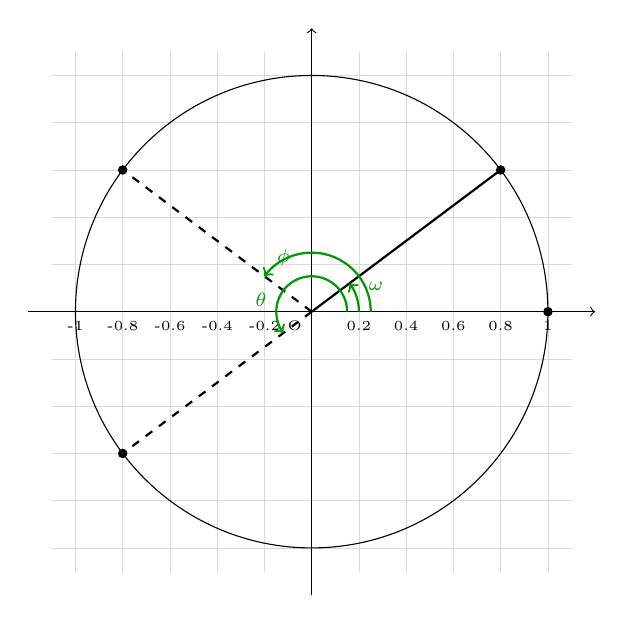
\begin{tikzpicture}[scale=3]
\draw[step=0.2,gray!30,very thin] (-1.1,-1.1) grid (1.1,1.1);
\draw[->] (-1.2,0) -- (1.2,0);
\draw[->] (0,-1.2) -- (0,1.2);
\draw (0,0) circle (1);

\foreach \x in {-1, -0.8, -0.6, -0.4, -0.2, 0.2, 0.4, 0.6, 0.8, 1}
    \node[below, font=\tiny] at (\x,0) {\x};
\node[below left, font=\tiny] at (0,0) {O};

% ray \omega at (0.8, 0.6)
\def\angw{36.87}
\draw[thick] (0,0) -- ({cos(\angw)}, {sin(\angw)});
\filldraw ({cos(\angw)}, {sin(\angw)}) circle (0.5pt);

% ray \phi at (-0.8, 0.6)
\def\angp{143.13}
\draw[thick, dashed] (0,0) -- ({cos(\angp)}, {sin(\angp)});
\filldraw ({cos(\angp)}, {sin(\angp)}) circle (0.5pt);

% ray \theta at (-0.8, -0.6)
\def\angt{216.87}
\draw[thick, dashed] (0,0) -- ({cos(\angt)}, {sin(\angt)});
\filldraw ({cos(\angt)}, {sin(\angt)}) circle (0.5pt);

% angle \omega
\draw[green!60!black, thick, ->] (0.2,0) arc (0:\angw:0.2);
\node[green!60!black, font=\scriptsize, above right] at (0.2, 0.05) {$\omega$};

% angle \phi
\draw[green!60!black, thick, ->] (0.25,0) arc (0:\angp:0.25);
\node[green!60!black, font=\scriptsize, above left] at (-0.05, 0.15) {$\phi$};

% angle \theta
\draw[green!60!black, thick, ->] (0.15,0) arc (0:\angt:0.15);
\node[green!60!black, font=\scriptsize, left] at (-0.15, 0.05) {$\theta$};

\filldraw (1,0) circle (0.5pt);
\end{tikzpicture}
\end{center}

\item Δύο γωνίες σχεδιασμένες στον τριγωνομετρικό κύκλο έχουν αντίθετα συνημίτονα, αν τα σημεία τομής της τελικής τους πλευράς με τον τριγωνομετρικό κύκλο είναι συμμετρικά ως προς τον άξονα $y'y$ ή ως προς την αρχή $O$ των αξόνων. Οπότε οι δύο γωνίες είναι παραπληρωματικές, δηλαδή $\phi = \pi - \omega$ ή διαφέρουν κατά $\pi$, οπότε $\theta = \pi + \omega$.
\end{alist}
